\section{Notch Filters}
\subsection{Radio Frequency Interference (RFI)}

Unfortunately, as the survey has progressed, we have become increasingly beset
by terrestrial, satellite and aircraft interference (see Figure~\ref{fig:intensity}). Aircraft interference is
sporadic enough in nature to flag out, but satellite and terrestrial interference is, however, more troublesome (see \fign{fig:intensity}). The effect on the data is noticeable up to 50$^{\circ}$ elevation, making post-measurement removal very difficult, if not impossible.

 To remedy this on the Northern receiver, we designed a set of narrowband notch filters (to reduce the effect of in-band RFI) and also increased the out-of band attenuation, by adding a second stage of band-defining filters. The resulting change of the passband can be seen in \fign{fig:passbands}. The effect on data quality (\fign{fig:intensityFiltering}) is noticeable and, with the 0.25s/pixel integration period used to produce these scans, RFI is no longer noticeable.

\begin{figure}
 \centering
\subfloat[][The C-BASS pass band before installing any additional filtering]{
 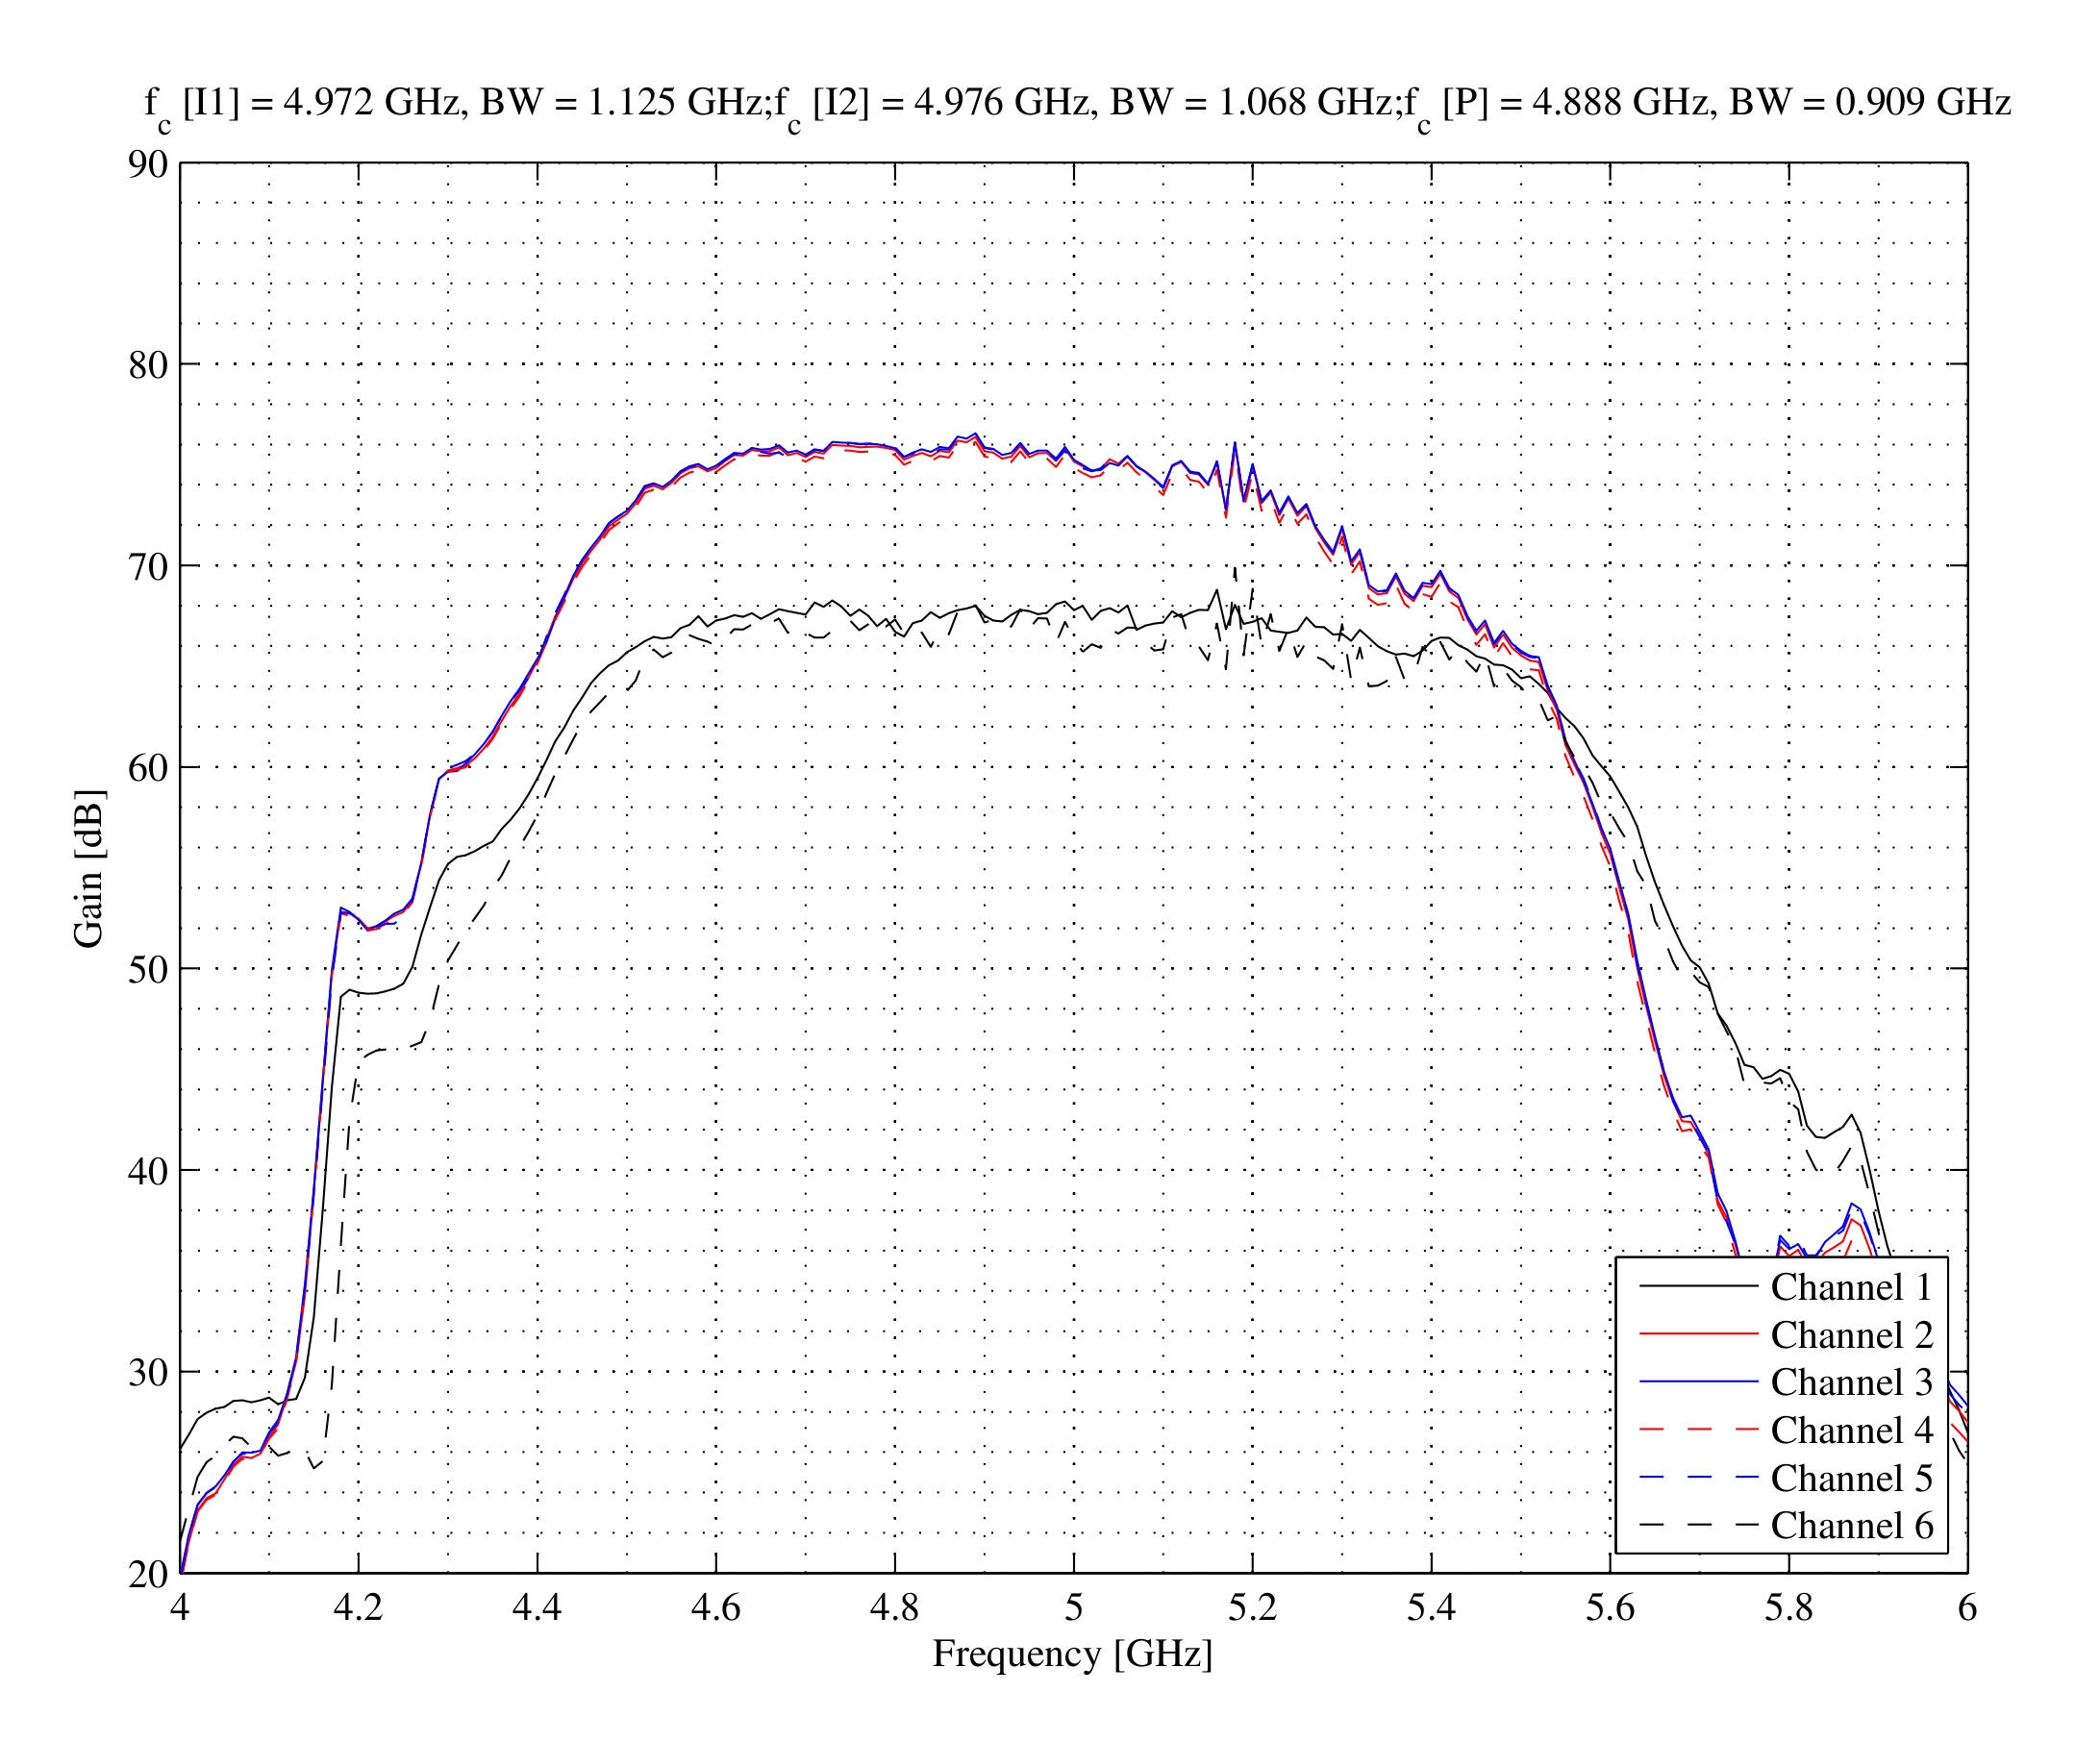
\includegraphics[height=0.4\textheight]{./images/NotchFilter/firstpassband.png}
}\\
\subfloat[][The C-BASS pass band after installing the Notch filters and additional Band pass filters]{
 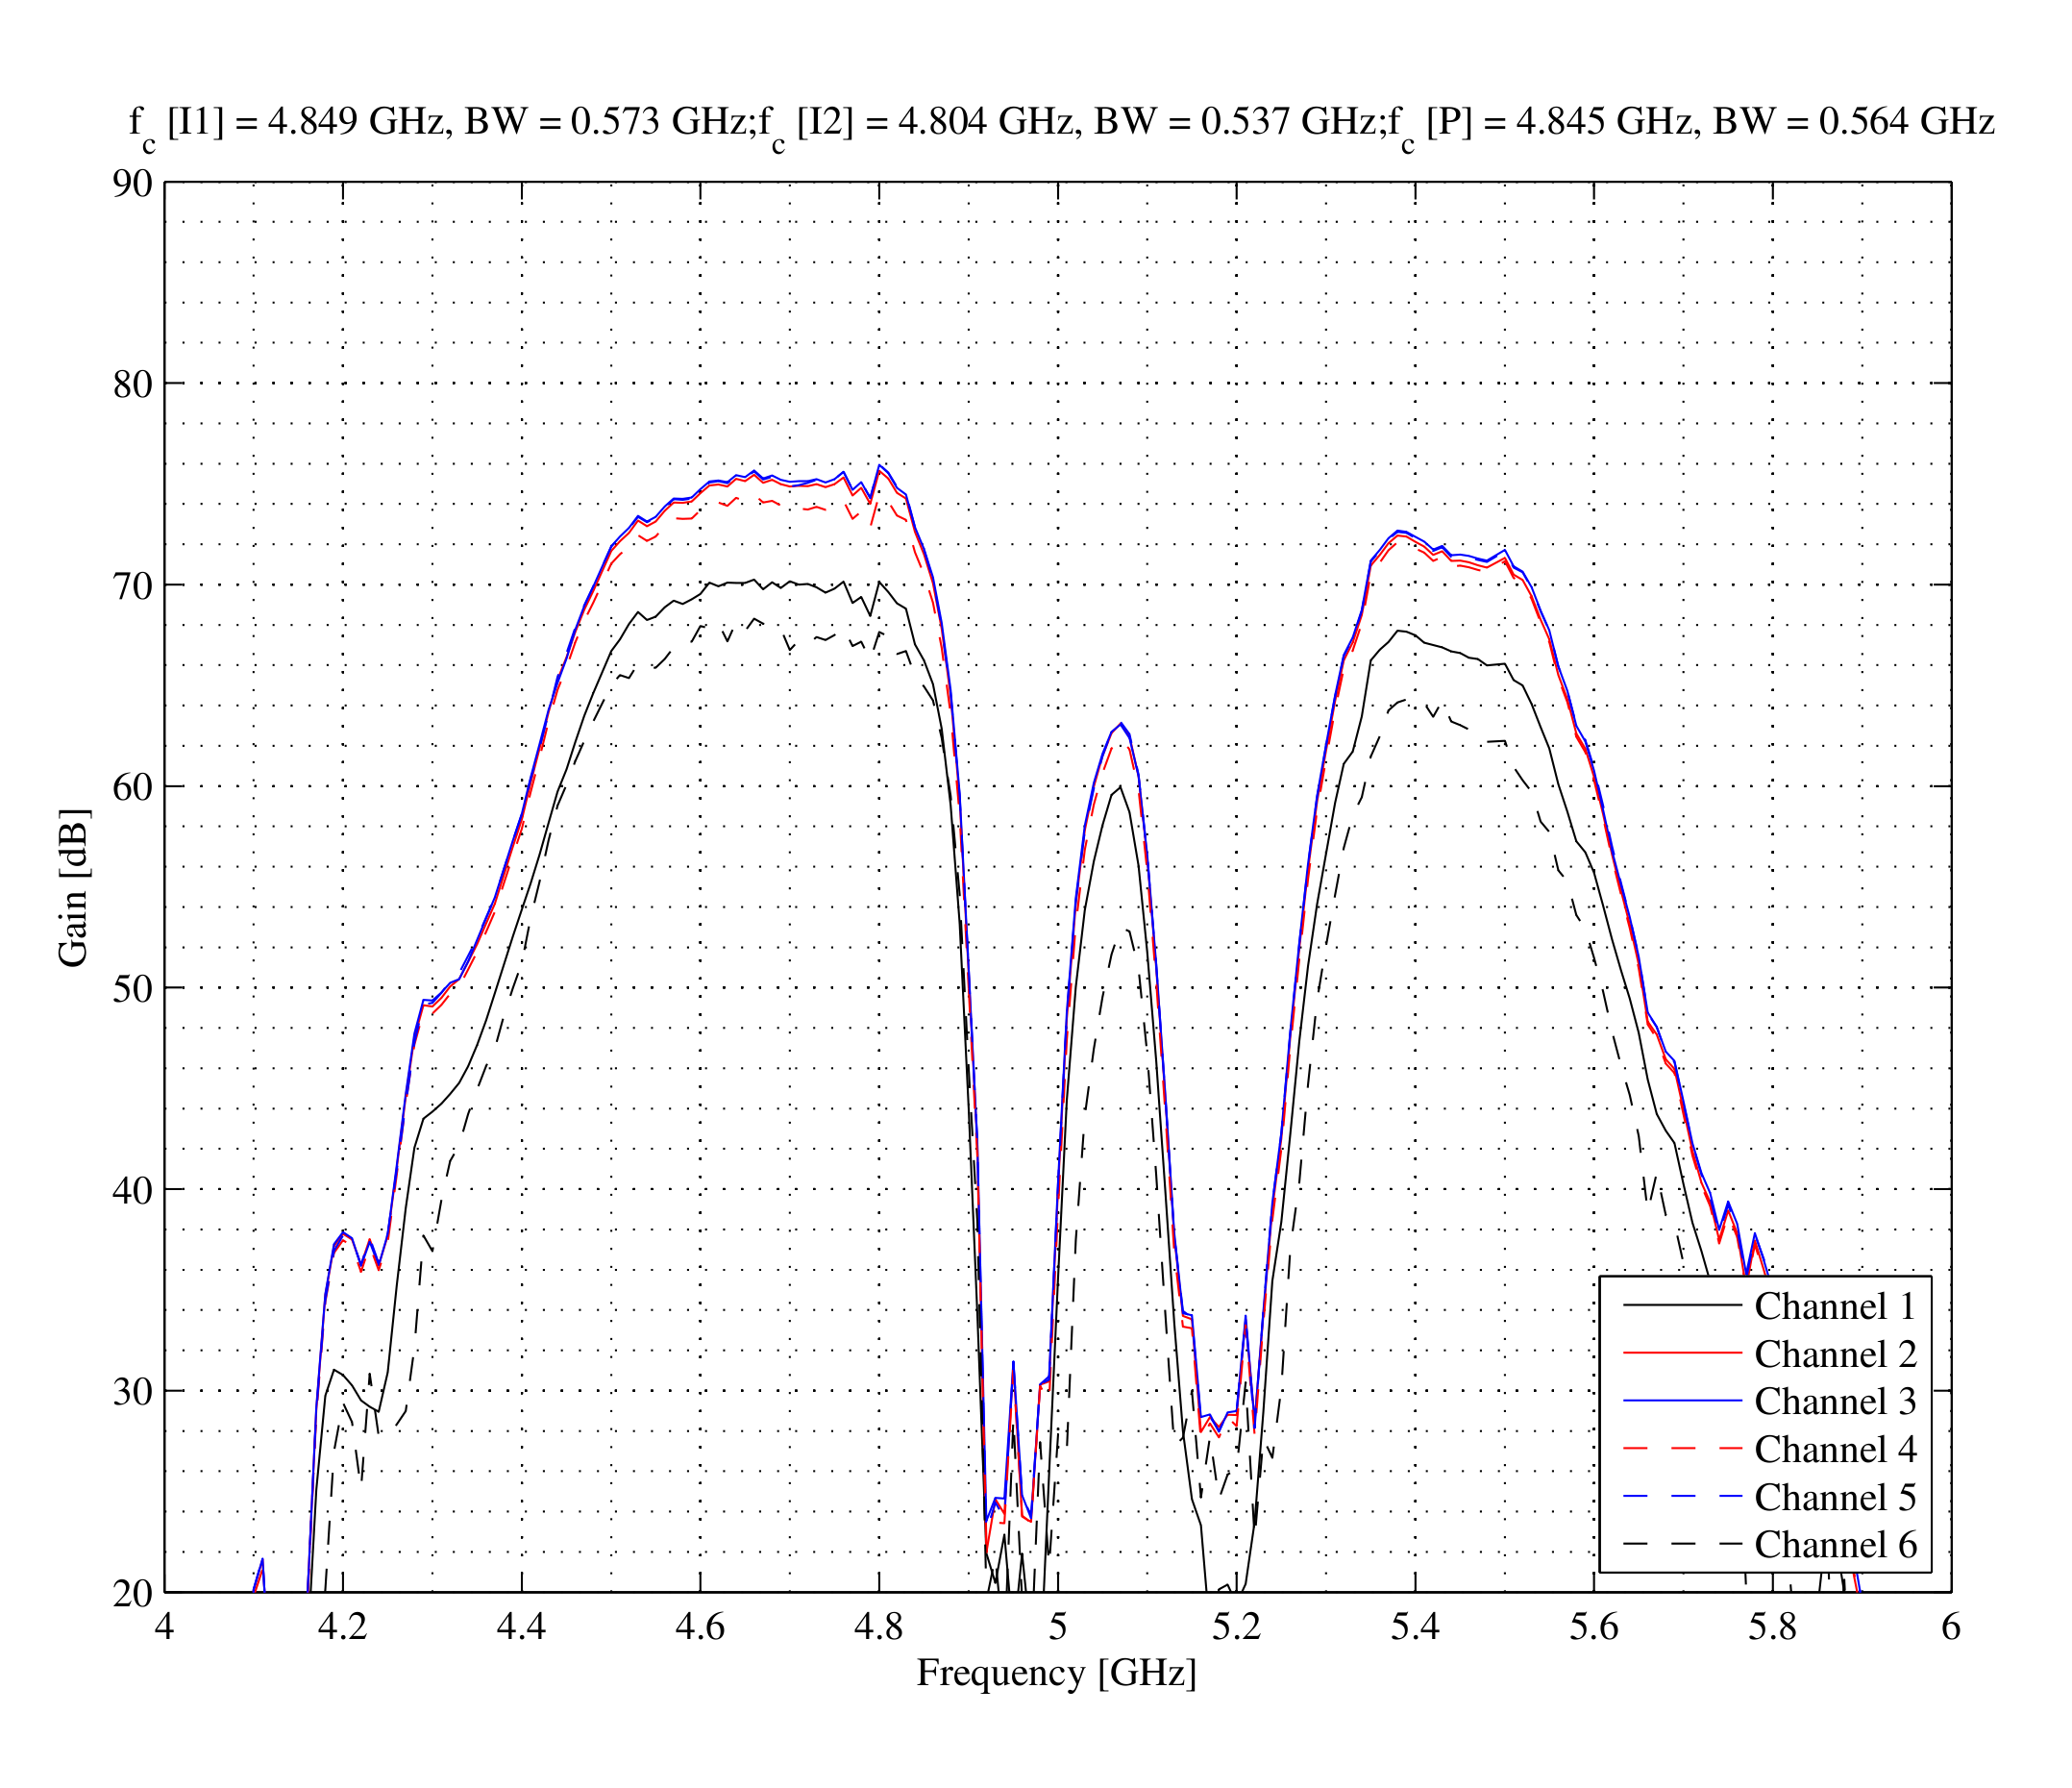
\includegraphics[height=0.4\textheight]{./images/NotchFilter/finalpassband.png}
}
 % firstpassband.pdf: 612x792 pixel, 72dpi, 21.59x27.94 cm, bb=
 \caption{C-BASS passband changes}
 \label{fig:passbands}
\end{figure}

\begin{figure}[ht]
 \centering
 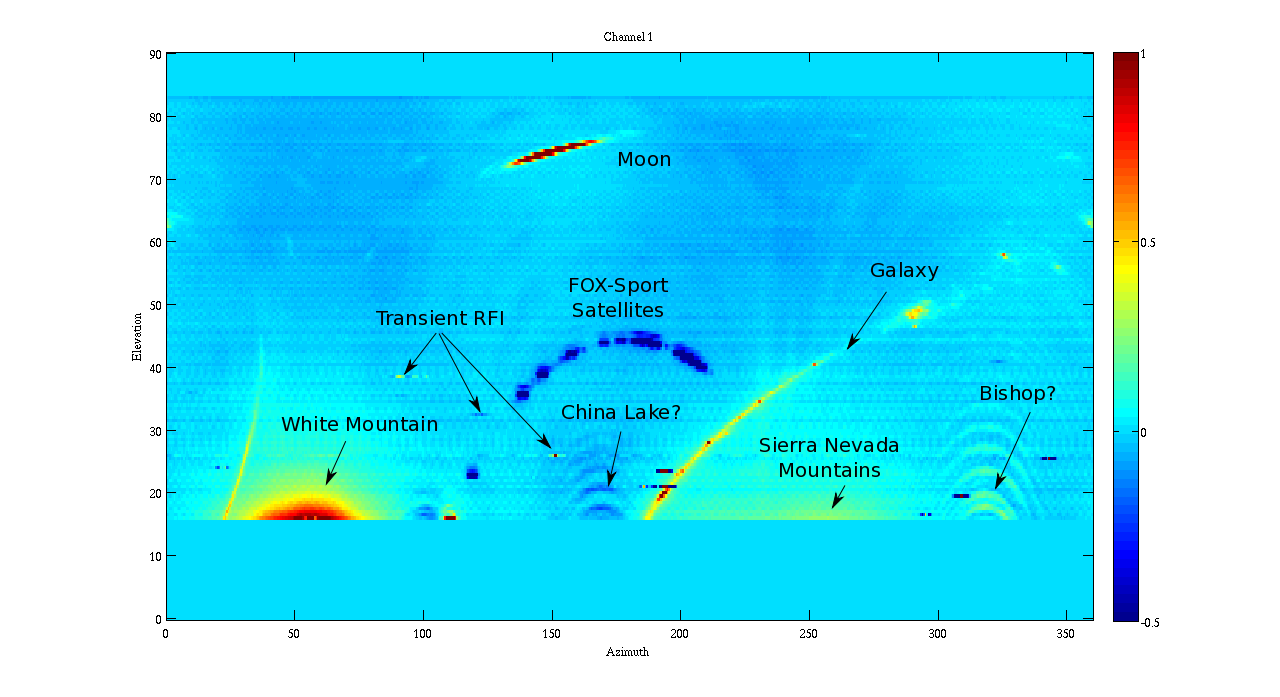
\includegraphics[width=\textwidth]{./images/NotchFilter/altazmapannotated.png}
 % altazmapi.png: 1280x701 pixel, 90dpi, 36.13x19.79 cm, bb=0 0 1024 561
 \caption{Annotated Intensity map (courtesy Oliver) of the sky as seen by the Owens Valley C-BASS antenna. Note the elevation extent of the diffraction patterns seen as a result of the terrestrial radiation }
 \label{fig:intensity}
\end{figure}


\begin{figure}
 \centering
\subfloat[][Sky before the installation of notch filters. Note the diffraction patterns produced by strong RFI sources detected in the antenna sidelobes]{
 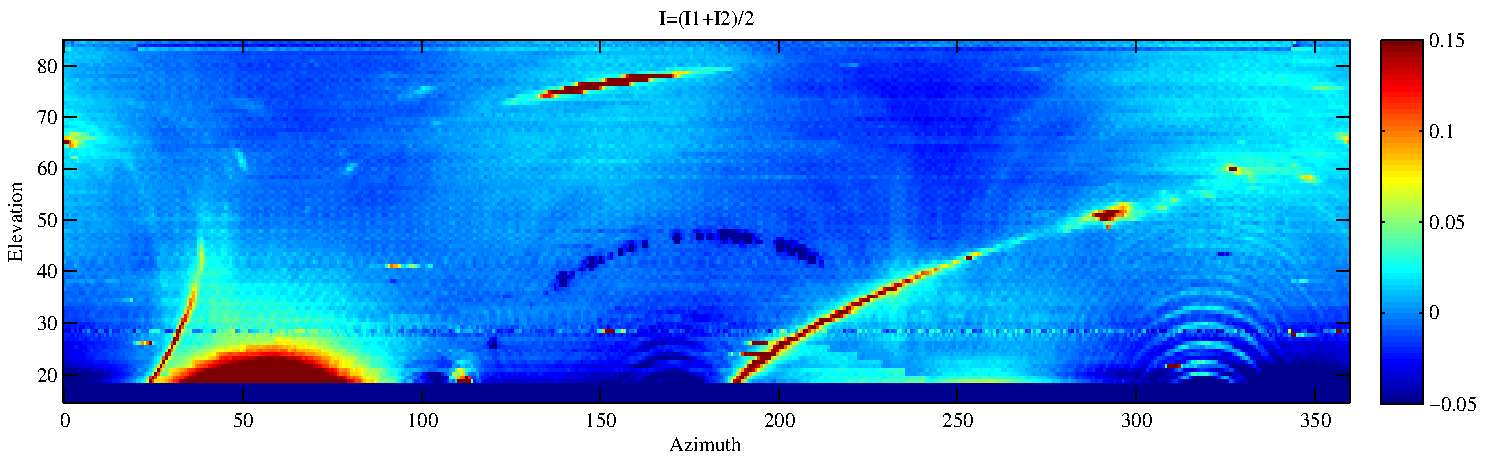
\includegraphics[width=\textwidth]{./images/NotchFilter/IntensityChannelBeforeNotch.pdf}
}\\
\subfloat[][Sky after the installation of notch filters. All terrestrial RFI aside from a strong source to the South ($180^{\circ}$~Azimuth) has been removed ]{
 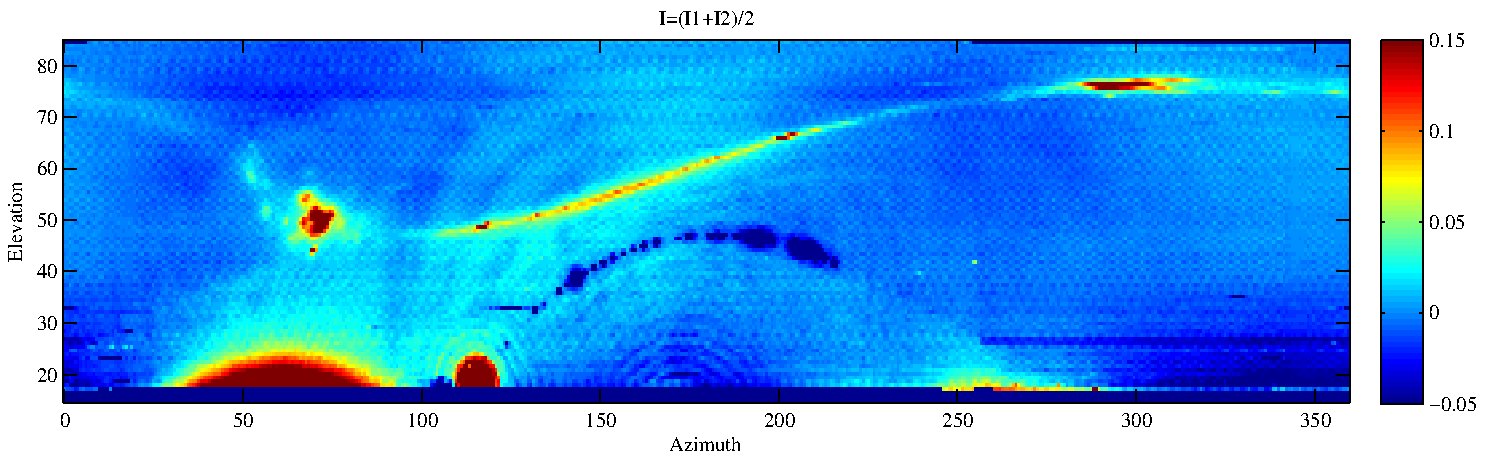
\includegraphics[width=\textwidth]{./images/NotchFilter/IntensityChannelAfterNotch.pdf}
}\\
\subfloat[][Sky after the installation of notch filters and additional band pass filters. All terrestrial radiation removed, and geostationary satellites are no longer visible]{
 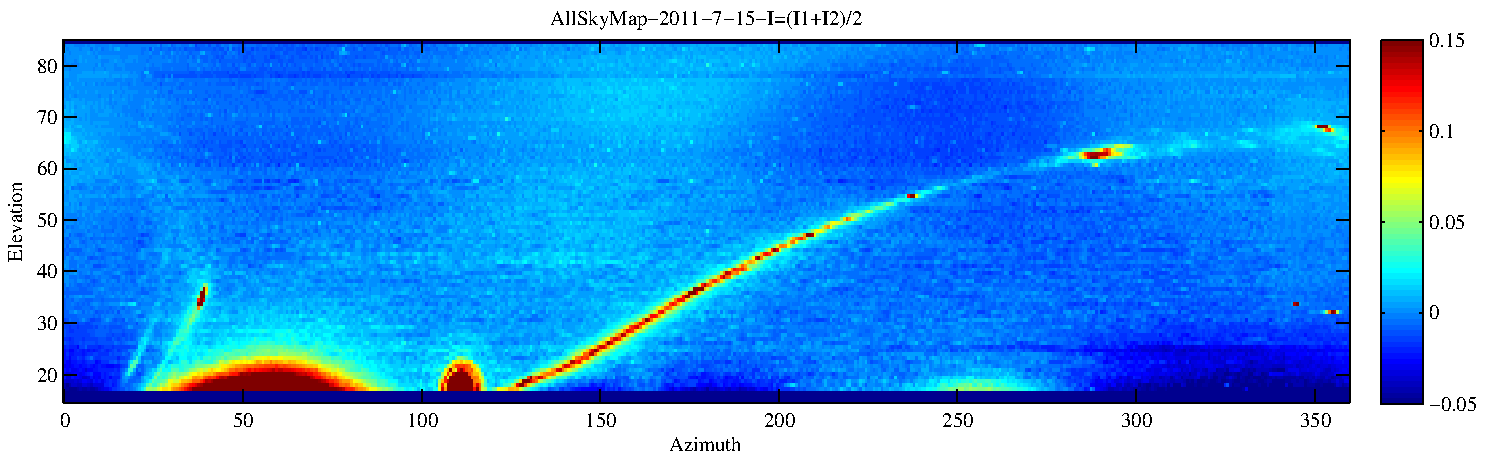
\includegraphics[width=\textwidth]{./images/NotchFilter/IntensityChannelAfterBPFandNotch.pdf}
}
\caption{Installing additional filtering: These images show the dramatic improvement in data quality brought about by the addition of notch filters and additional band defining filters in the C-BASS RF path}
\label{fig:intensityFiltering}
 % IntensityChannelBeforeNotch.pdf: 713x220 pixel, 72dpi, 25.15x7.76 cm, bb=
\end{figure}


\begin{figure}
 \centering
\subfloat[][Radio Frequency Interference as captured by a spectrum analyser attached to the output of the C-BASS cryostat. We think the 4.79~GHz spike is sporadic and does not require filtering]{
 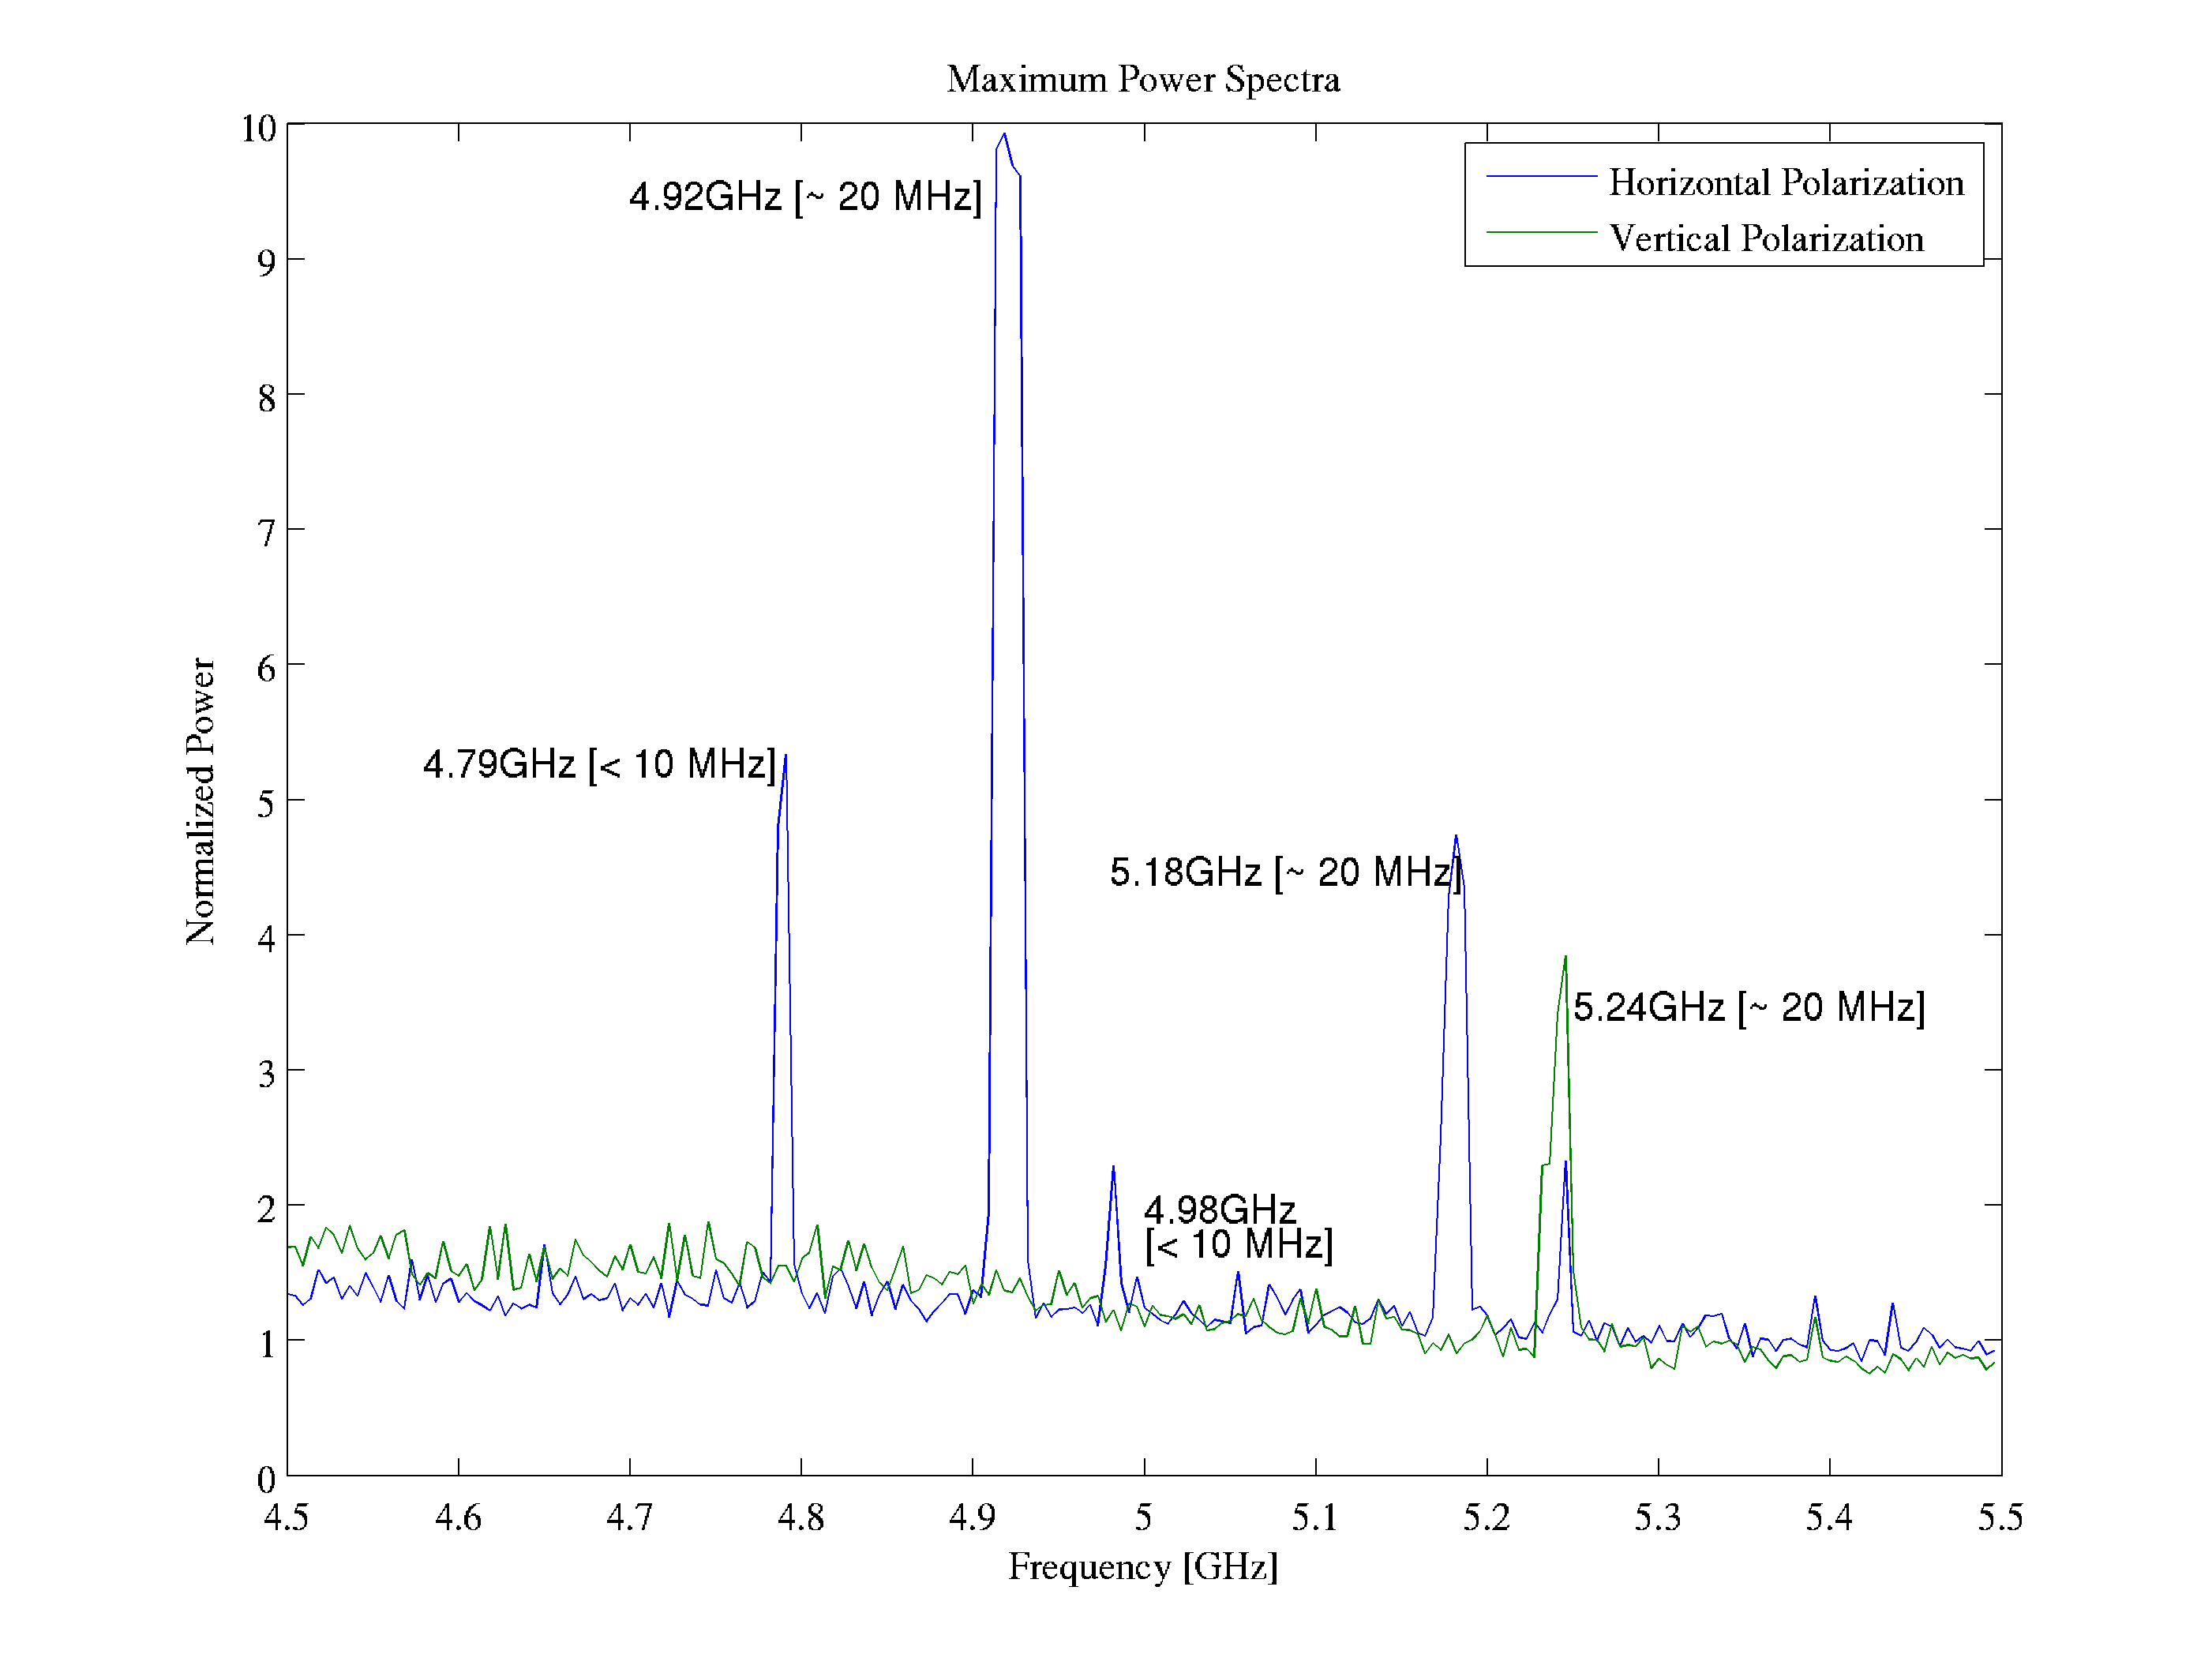
\includegraphics[height=0.4\textheight]{./images/NotchFilter/RFI/norm_max_rfi.png}
}\\
 % norm_max_rfi.png: 2802x2100 pixel, 350dpi, 20.33x15.24 cm, bb=0 0 576 432
 \subfloat[][Spectra of geostationary satellites]{
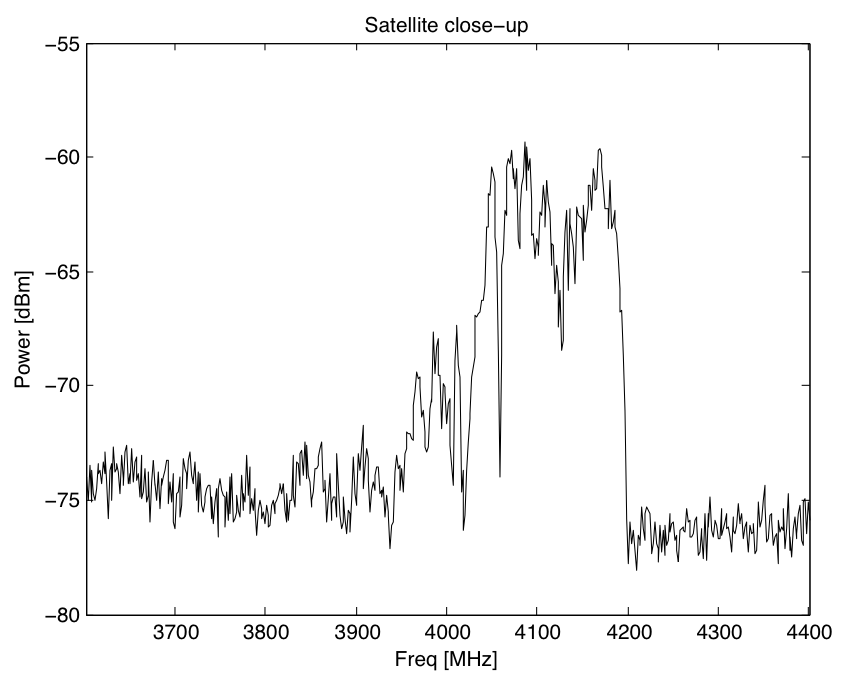
\includegraphics[height=0.4\textheight]{./images/NotchFilter/RFI/figs-satellite.png}}
\caption{}
 \label{fig:RFImaxHold}
\end{figure}




\clearpage
% \begin{figure}
%  \centering
%  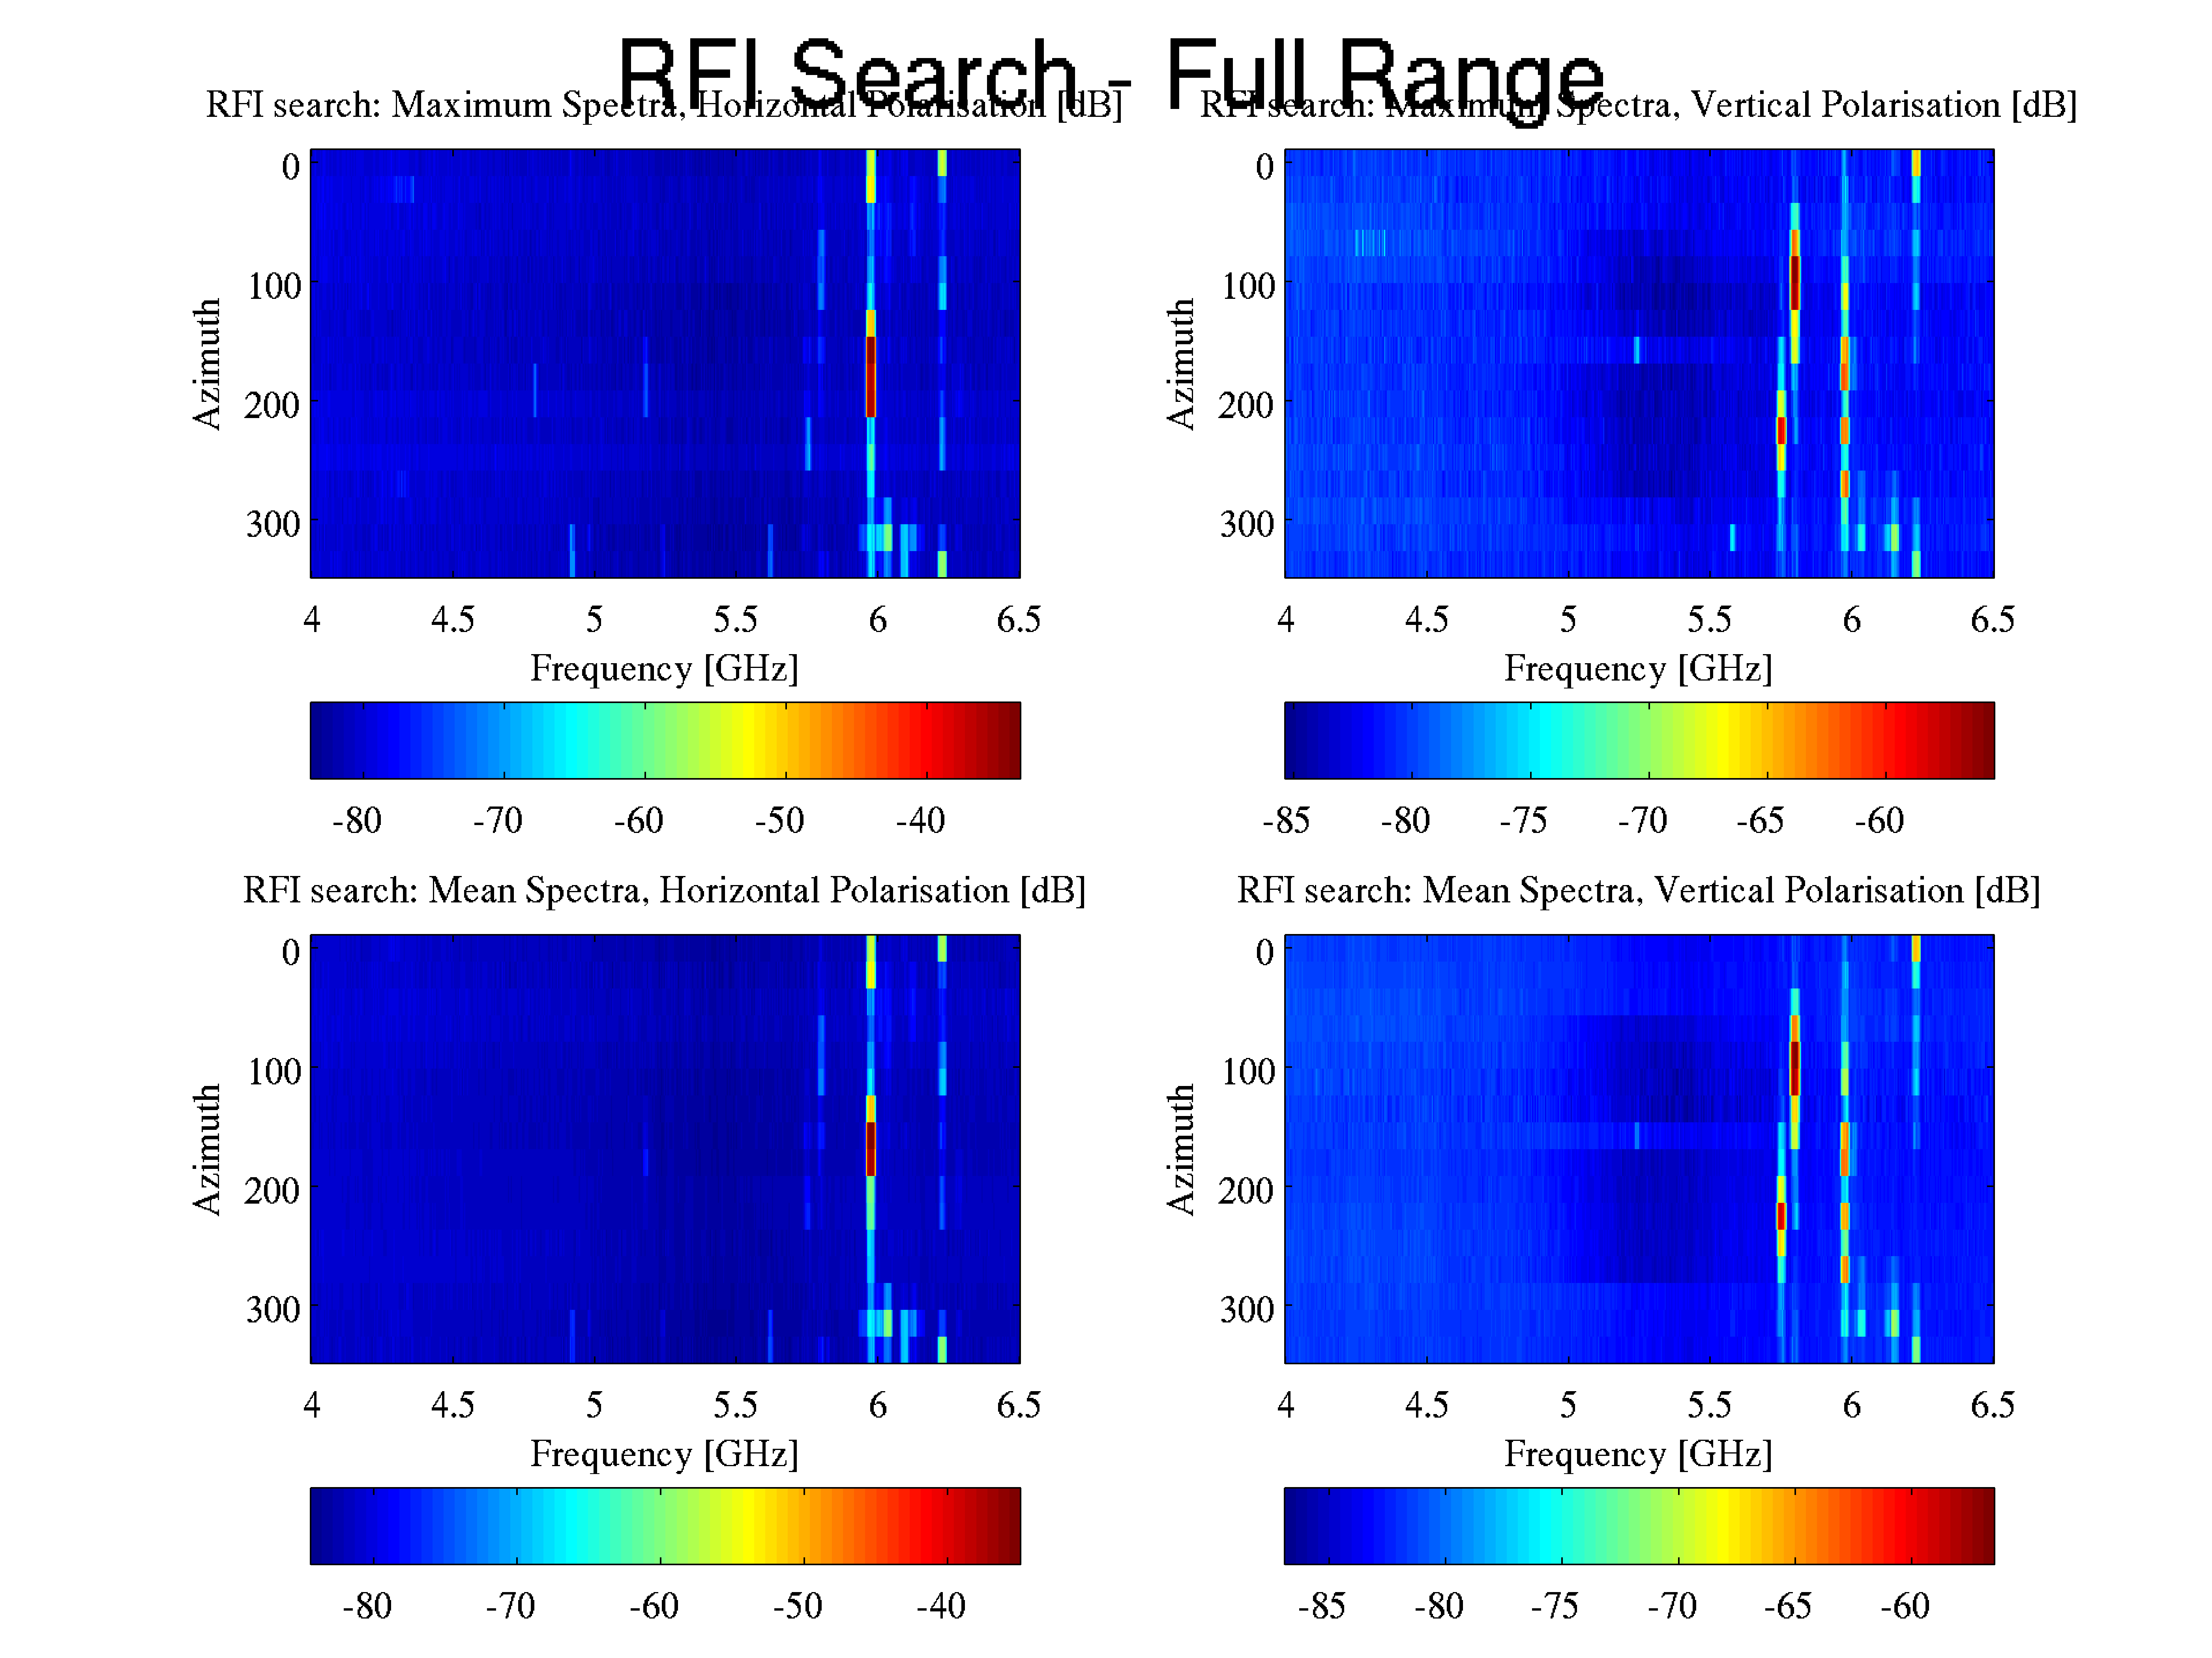
\includegraphics{./images/NotchFilter/RFI/rfi_full_range.png}
%  % rfi_full_range.png: 5605x4200 pixel, 700dpi, 20.34x15.24 cm, bb=0 0 577 432
%  \caption{Radio Frequency Interference as seen at Owens Valley with directionality}
%  \label{fig:RFI}
% \end{figure}


\subsection{Filter Design}

\subsection{Specifications}
An obvious solution to this is to design a set of very high Q ($Q=\frac{f_{c}}{\Delta f}$) notch filters. A cursory examination of Figure~\ref{fig:RFImaxHold} suggests that each RFI band is approximately 25~MHz wide, which at 5~GHz requires a Q of 200. This is a challenging task.

However upon more careful examination of Figure~\ref{fig:RFImaxHold}, it is clear that some relaxation of this is possible. Each of the major RFI bands (i.e 4.92~GHz and 5.18~GHz) has a second proximate RFI peak, which could be included into a single notch filter. To attenuate both of these a stop band of ~80~MHz is required. This is an achievable goal.

\subsection{Design}

High Q filter design using microstrip, is usually accomplished using resonance structures placed parallel to a microstrip transmission line, with electromagnetic coupling between the two. The dimensions of these structures can be adjusted to resonate at the frequency of interest. Alternatively band pass filters can be constructed in a similar fashion by placing these resonating structures in series with the transmission line.

Since this was our first foray into the world of resonance filter designs we looked for a simple resonating structure which would be easy to 'tune'. The design we chose (\cite{splitRingClassic} )is shown in Figure~\ref{fig:squareRingResonator}.

\begin{figure}[ht]
 \centering
 \subfloat[Square Resonator]{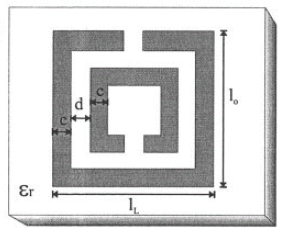
\includegraphics[width=0.4\textwidth]{./images/NotchFilter/squareRingResonator.png} \label{fig:squareResonator}}
 \subfloat[Circular Resonator]{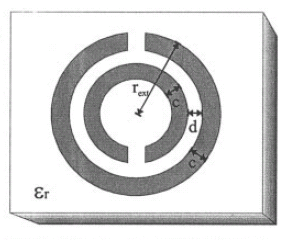
\includegraphics[width=0.4\textwidth]{./images/NotchFilter/circularRingResonator.png} \label{fig:circleResonator}}\\
 \subfloat[Manufactured Bandstop filter with a series of differently tuned square resonator structures]{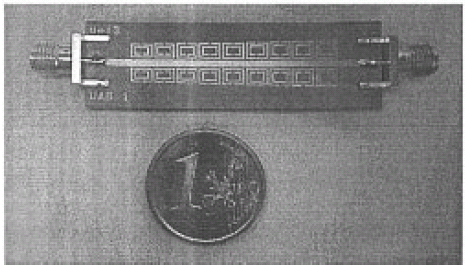
\includegraphics[width=0.4\textwidth]{./images/NotchFilter/Design1.png} \label{fig:design1} } 
\subfloat[S21 Bandstop filter Result- See SRR plot]{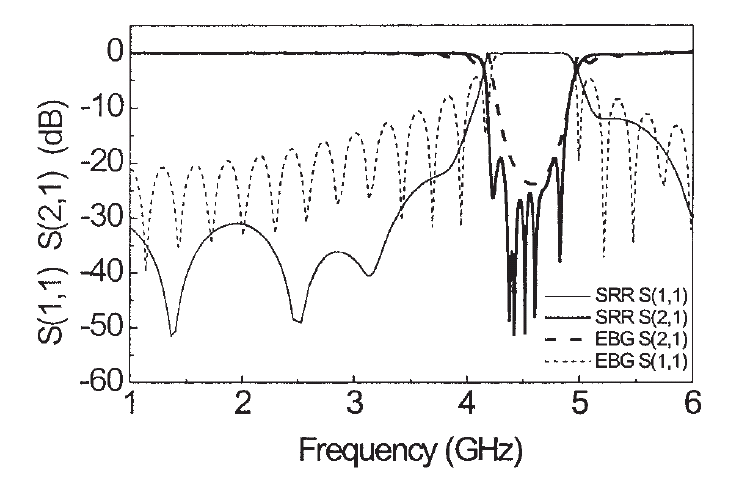
\includegraphics[width=0.4\textwidth]{./images/NotchFilter/s21.png} \label{fig:s21design1} } 
 \caption{Possible resonance structures for the notch filter \cite{splitRingClassic}. These diagrams show the dimensions that can be adjusted. We chose to pursue the square type resonance structure \ref{fig:squareResonator}}
 % squareRingResonator.png: 287x238 pixel, 72dpi, 10.12x8.40 cm, bb=0 0 287 238
 \label{fig:squareRingResonator}
\end{figure}

We used these resonators to design 3 initial filters for 4.65~GHz, 4.70~GHz and 4.75~GHz. This we felt would allow use to check that the filter behaved as the simulations predicted across a small range of frequencies.
\clearpage
\subsection{Manufacture and Testing}

\begin{figure}
 \centering
 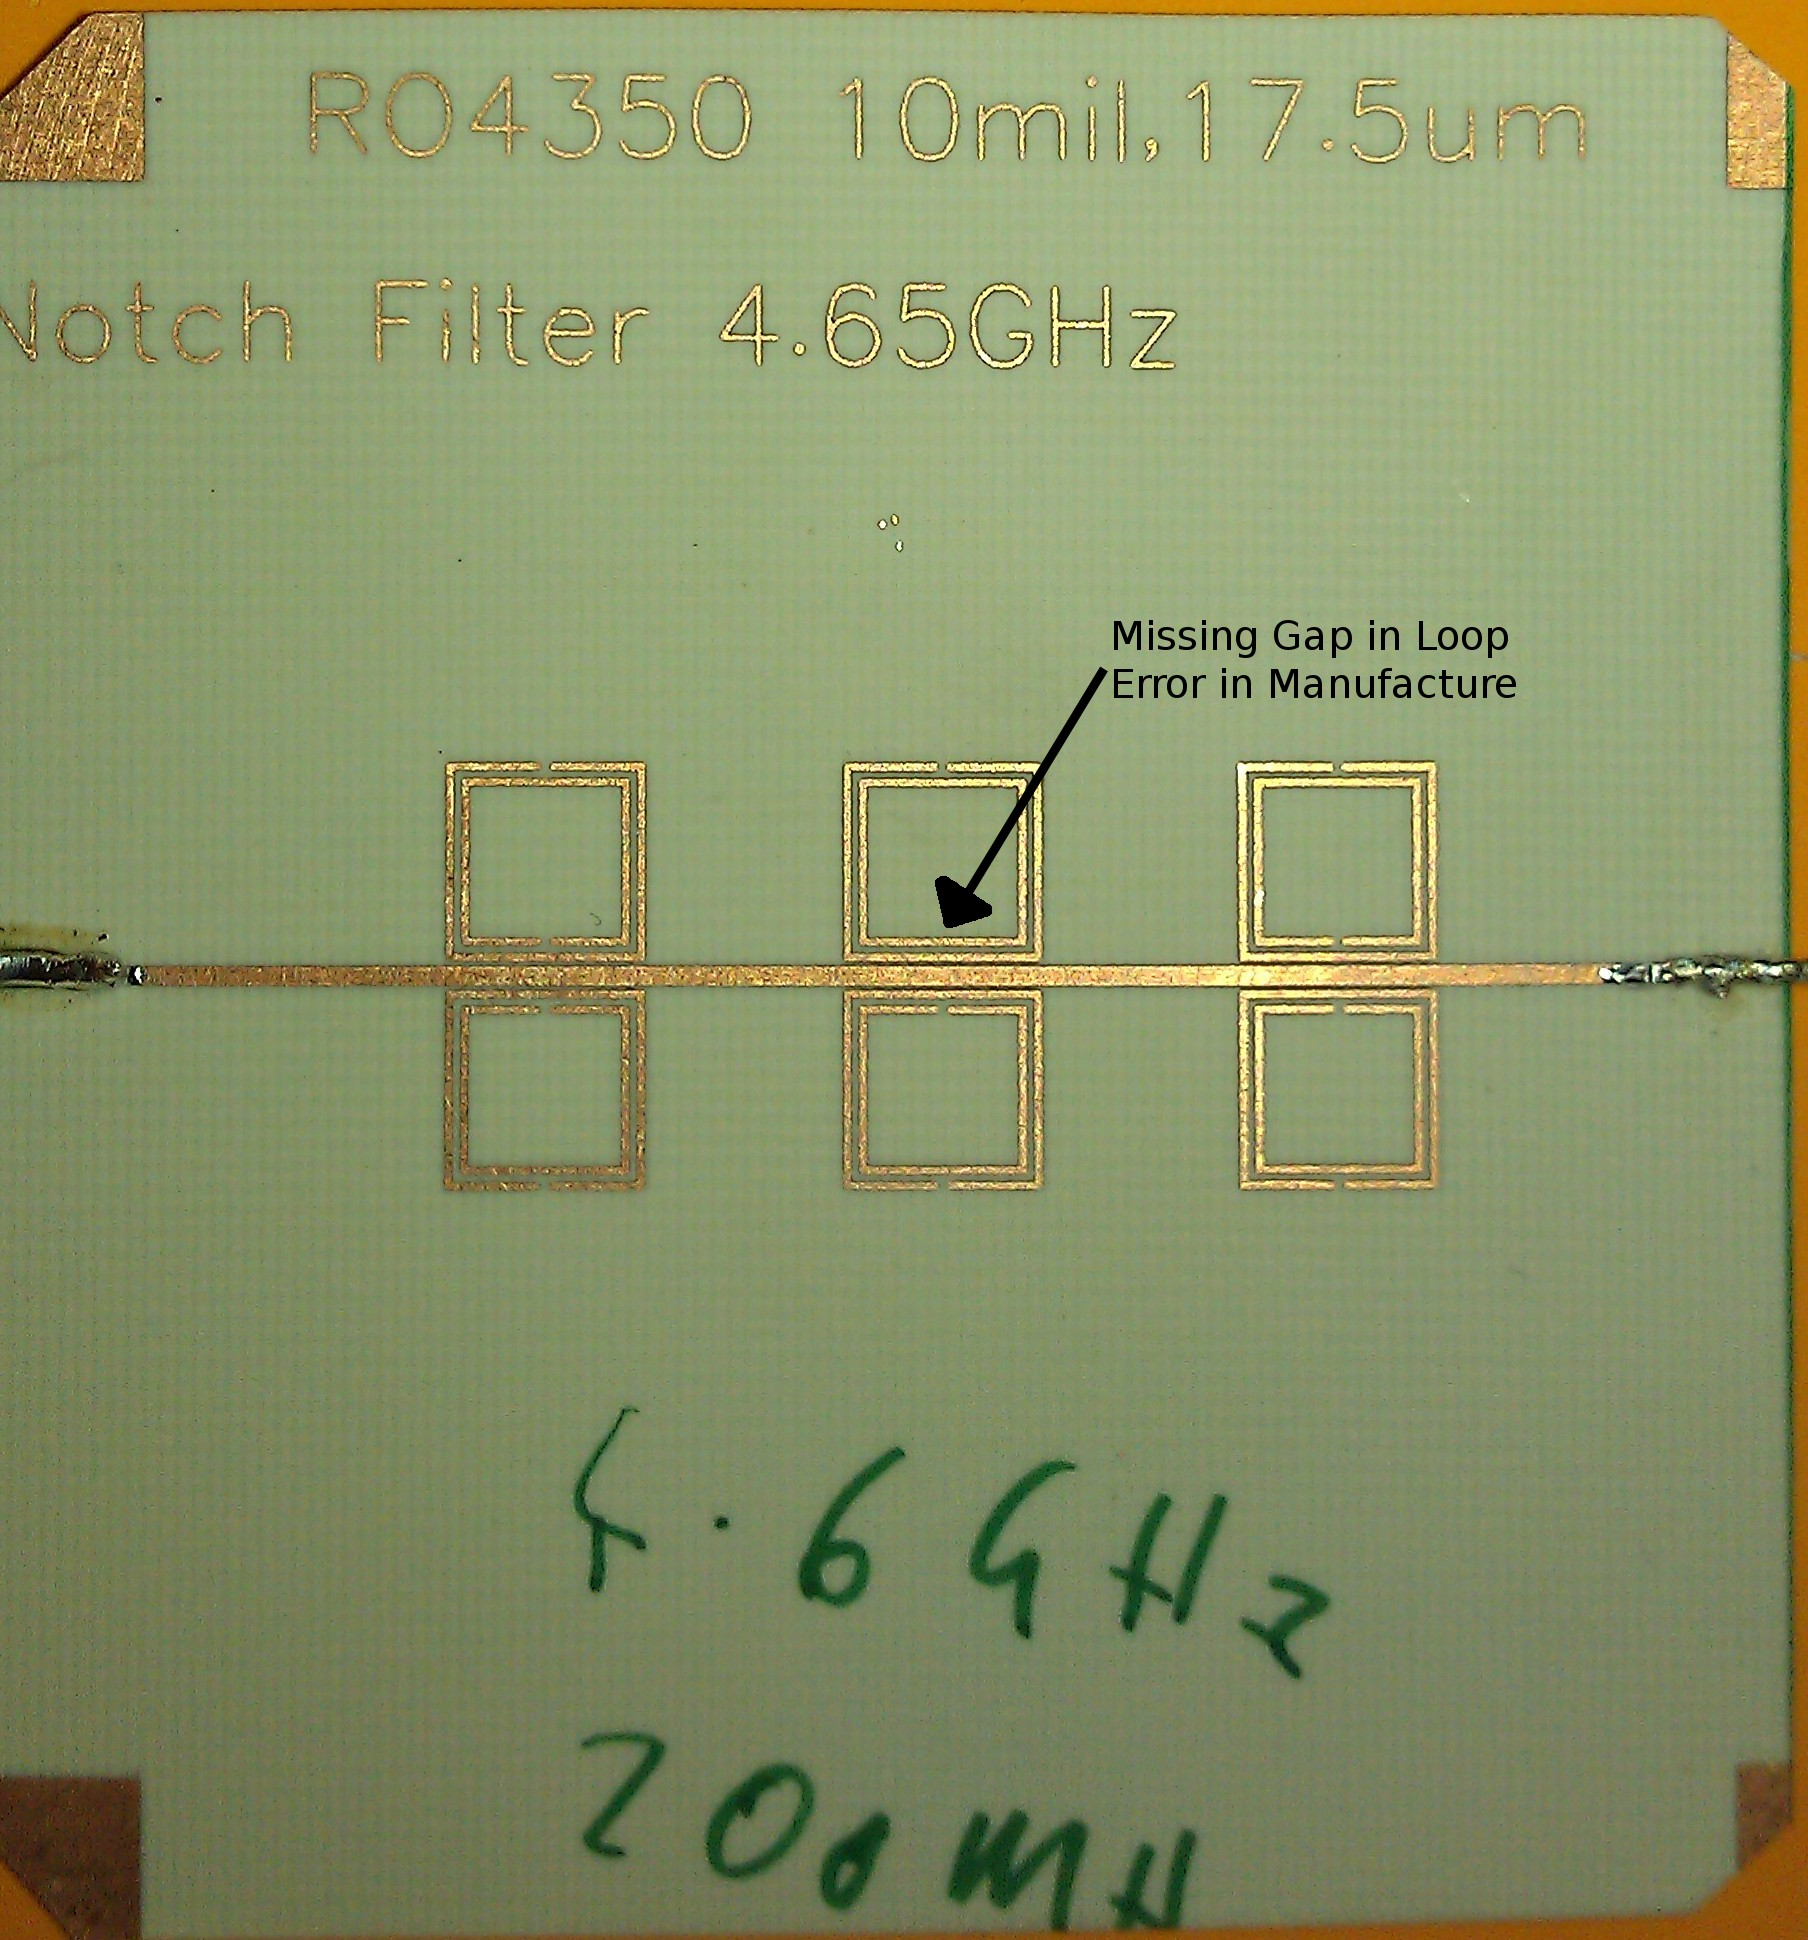
\includegraphics[width=0.5\textwidth]{./images/NotchFilter/IMAG0148.jpg}
 % IMAG0148.jpg: 1808x1940 pixel, 72dpi, 63.78x68.44 cm, bb=0 0 1808 1940
 \caption{The manufactured 4.65~GHz notch filter. Used Rogers RO4350 10mil (Er=3.66) with 17.5um Copper layers for manufacture. Note the error in manufacture. This produced an additional notch feature (apparent in Figure~\ref{fig:MeasuredResults}) at ~10\% higher frequency than the central notch feature. This has been corrected}
 \label{fig:4_65GHzFilter}
\end{figure}


\begin{figure}
 \centering
 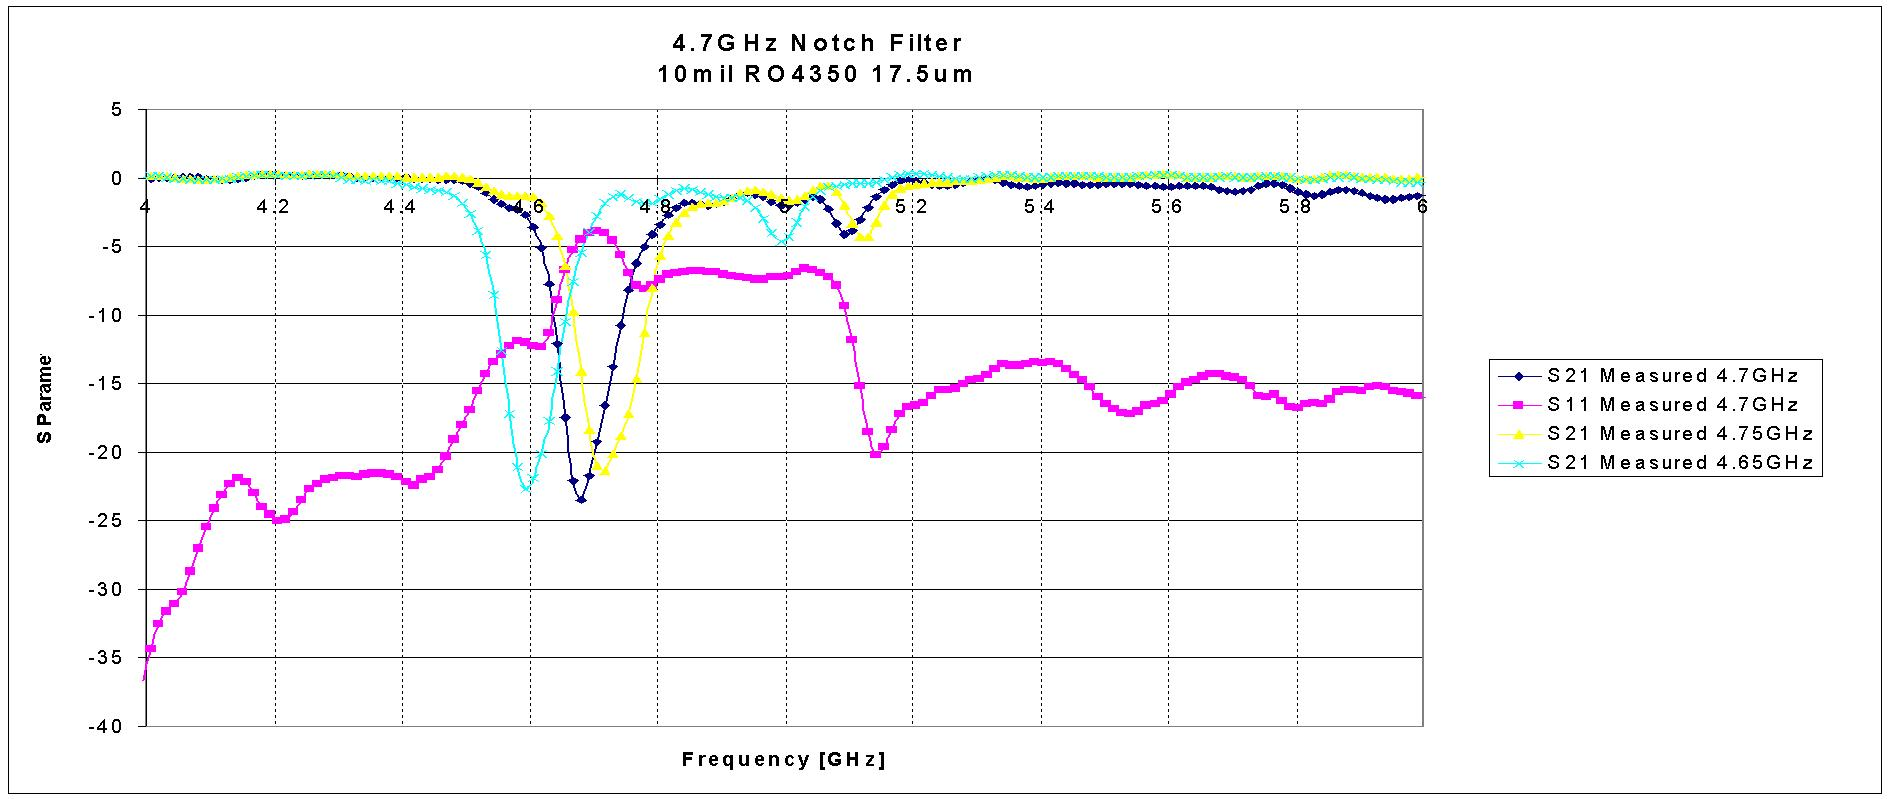
\includegraphics[width=\textwidth]{./images/NotchFilter/MeauredResults.JPG}
 % MeauredResults.JPG: 1890x799 pixel, 96dpi, 50.01x21.14 cm, bb=0 0 1418 599
 \caption{Measured Results of the three square ring resonator structures. We see the additional feature ~10\% higher in frequency caused by the error in manufacture (see Figure~\ref{fig:4_65GHzFilter}) in all three of the designs. We also see that the central notch behaves as we expect although they are approximately 50~MHz lower than the simulations predict}
 \label{fig:MeasuredResults}
\end{figure}

\clearpage
\subsection{Cooling the Filters}

We expected the filter bandwidth to improve at lower temperatures, since most of the loss was resistive loss in the Copper. To test this we initially cooled the design with liquid nitrogen, however we found that the liquid nitrogen effected the central response by changing the dielectric constant of the region directly above the resonator structures.

We decided then to conduct the test in the Oxford test cryostat and achieved the following results.

\begin{figure}[ht]
 \centering
 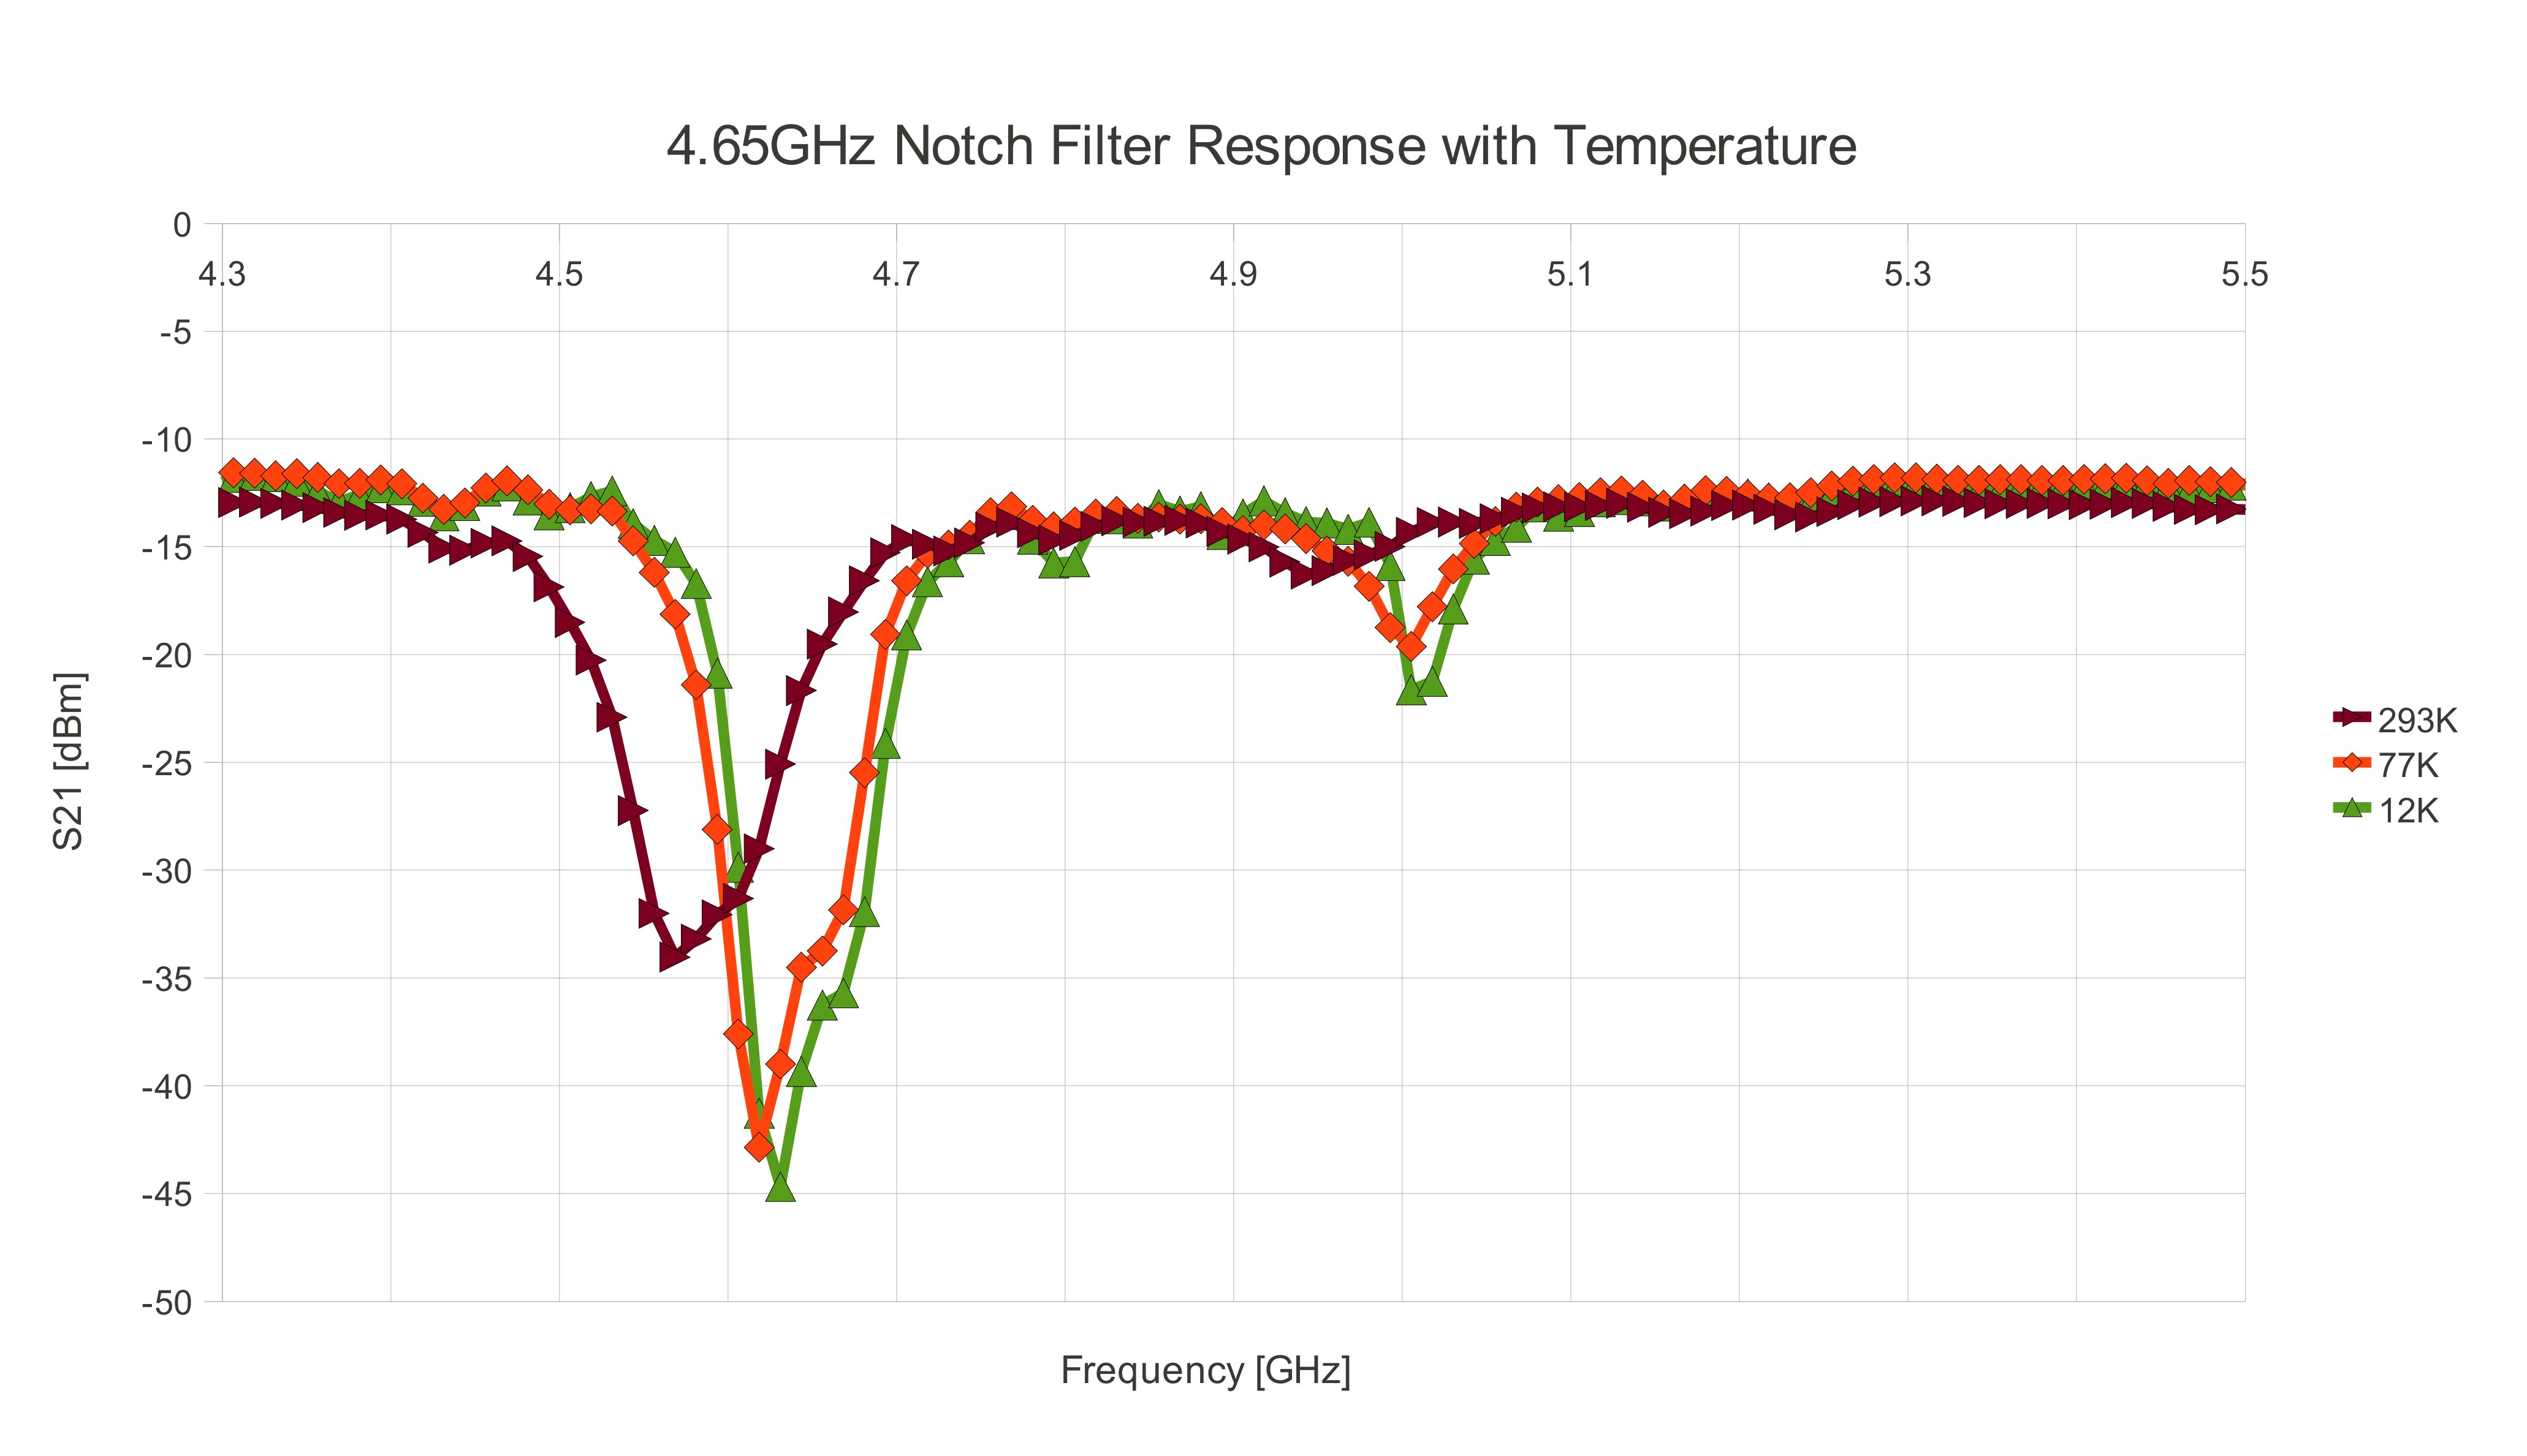
\includegraphics[width=\textwidth]{./images/NotchFilter/CoolingResponse.jpg}
 % CoolingResponse.pdf: 595x842 pixel, 72dpi, 20.99x29.70 cm, bb=0 0 595 842
 \caption{Cooling the Filter in the test cryostat. Note the additional notch feature becomes more pronounce when cooled.}
 \label{fig:coolingResponse}
\end{figure}
\clearpage

\subsection{Filter Installation at Owens Valley Antenna}

The RFI notch filters were installed at the Owens Valley antenna on the 7~May~2011 (see \fign{fig:cryostatInstall}). The filters have successfully suppressed the RFI shown in \fign{fig:RFImaxHold}. The transmission through the cryostat can be seen in \fign{fig:cryostatTransmission}.

\begin{figure}
 \centering
 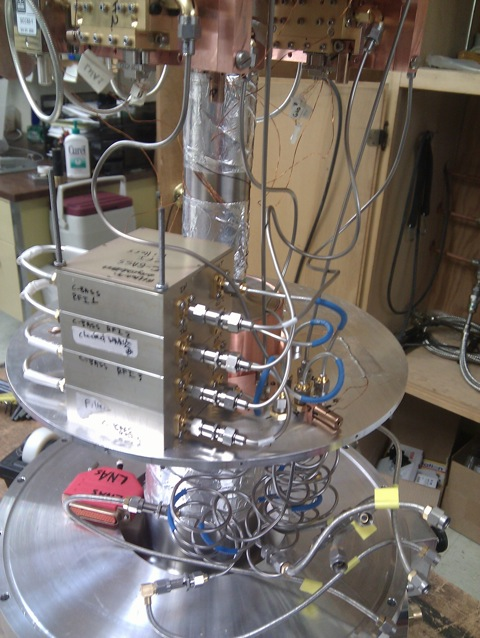
\includegraphics[height=0.6\textheight]{./images/NotchFilter/cryostatInstall.jpg}
 % cryostatInstall.jpg: 480x638 pixel, 72dpi, 16.93x22.51 cm, bb=0 0 480 638
 \caption{The notch filters installed in the cryostat at Owens Valley}
 \label{fig:cryostatInstall}
\end{figure}

\begin{figure}
 \centering
 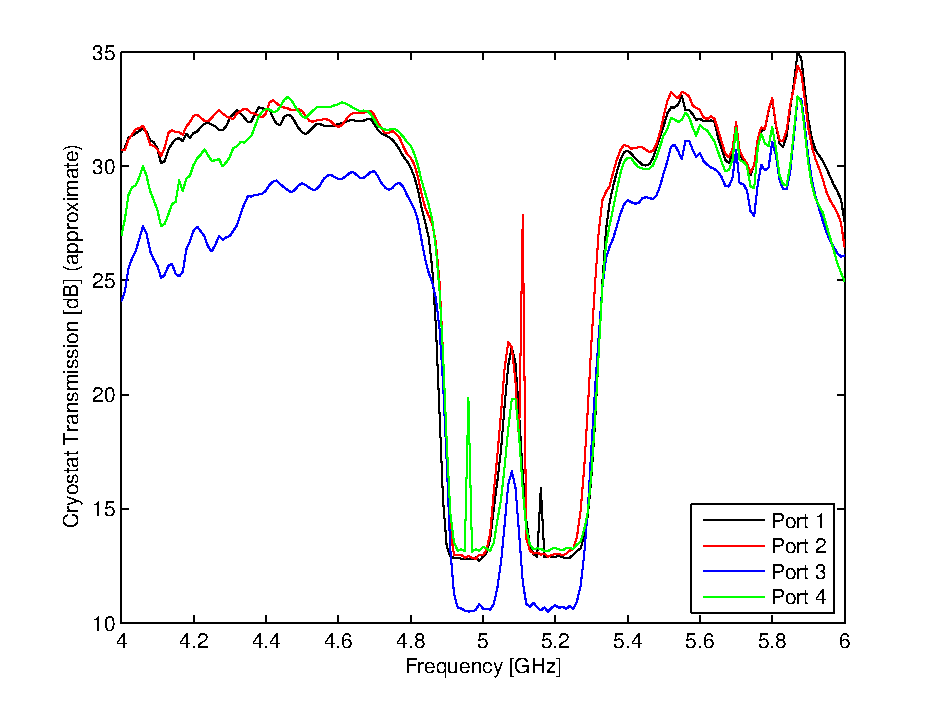
\includegraphics[width=0.6\textwidth]{./images/NotchFilter/CryostatTransmission.pdf}
 % cryostatInstall.jpg: 480x638 pixel, 72dpi, 16.93x22.51 cm, bb=0 0 480 638
 \caption{Transmission through the cryostat after the installation of the notch filters. The two stop bands prevent incoming RFI from contaminating the signal}
 \label{fig:cryostatTransmission}
\end{figure}
% 
%   \subsection{Current Ongoing Work}
% 
%   Future work has included manufacturing filters appropriate to mitigating the Owens Valley RFI seen in Figure~\ref{fig:RFImaxHold}. An image of one of these can be seen in Figure~\ref{fig:newDesign}.
%   \begin{figure}[ht]
%   \centering
%   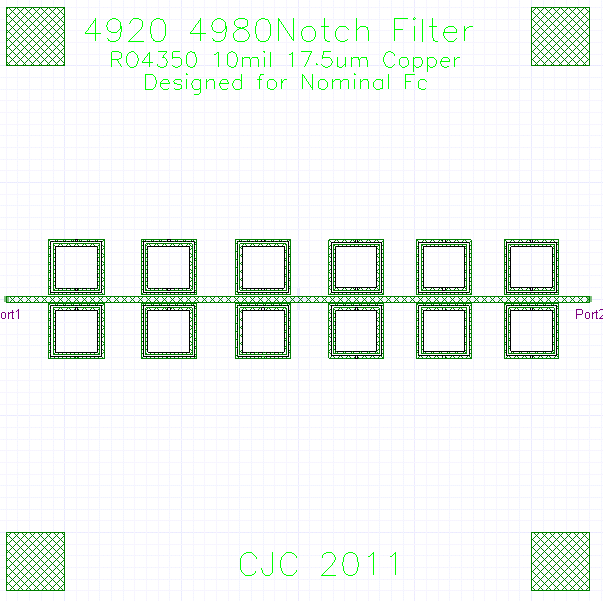
\includegraphics[width=0.6\textwidth]{./images/NotchFilter/NewDesign.png}
%   % NewDesign.png: 603x601 pixel, 72dpi, 21.27x21.20 cm, bb=0 0 603 601
%   \caption{The new multi frequency notch filter for 4920~MHz and 4980~MHz RFI seen in Figure~\ref{fig:RFImaxHold}. Similar designs exist for the 5180~MHz and 5240~MHz. All have several variations in the central frequency to allow the best version to be selected. It should be noted that I have a little concern about the effect that we will see when we have the first and last resonators so close to the box wall. Simulations don't suggest any issues, but tests still need to be conducted to be sure. }
%   \label{fig:newDesign}
%   \end{figure}

\clearpage

\subsection{Other Possibilities}

High temperature superconducting filters \cite{splitRingHTS}, would achieve much higher Q values, allowing us to design filters for each of the RFI features. However the manufacture process is complicated, and in addition would be a new method for the Physics department. We are however currently pursuing this, and should have preliminary results in the next few weeks.

The other possibility is to switch over to a digital polarimeter. There would be some time delay in getting this implemented and working, however it would synergise efforts when rolling out the South African antenna. 
% \begin{figure}
%  \centering
%  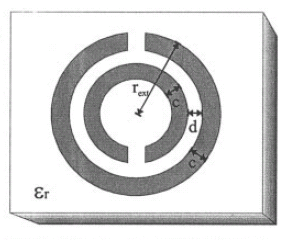
\includegraphics{./images/NotchFilter/circularRingResonator.png}
%  % circularRingResonator.png: 302x240 pixel, 72dpi, 10.65x8.47 cm, bb=0 0 302 240
%  \caption{Circular Ring Resonator}
%  \label{fig:circleRingResonator}
% \end{figure}













\clearpage